\documentclass{article}
\usepackage{amsthm, amsmath, tikz}
\usepackage[margin=1in]{geometry}
\begin{document}
    \noindent\textbf{Math 327 Homework 2}\hfill Anchu A. Lee\\\\
    
    \noindent\textbf{2.4}
    \begin{enumerate}
        \item $S = \{(1,1),(1,2),(1,3),(1,4),(1,5),(1,6),(2,1),(2,2),(2,3),(2,4),(2,5),(2,6)\\
               (3,1),(3,2),(3,3),(3,4),(3,5),(3,6),(4,1),(4,2),(4,3),(4,4),(4,5),(4,6)\\
               (5,1),(5,2),(5,3),(5,4),(5,5),(5,6),(6,1),(6,2),(6,3),(6,4),(6,5),(6,6)\}$
        \item $S = \{x, y \mid 0\leq x \leq 6, 0 \leq y \leq 6\}$
    \end{enumerate}
    \textbf{2.6}\\
        $S = \{A_1A_2, A_1A_3, A_1A_4, A_2A_3, A_2A_4, A_3A_4\}$\\\\
    \textbf{2.8}
    \begin{enumerate}
        \item $A = \{(3,6),(4,5),(4,6),(5,4),(5,5),(5.6),(6,3),(6,4),(6,5),(6,6)\}$
        \item $B = \{(1,2),(2,1),(2,2),(2,3),(2,4),(2,5),(2,6),(3,2),(4,2),(5,2),(6,2)\}$
        \item $C = \{(5,1),(5,2),(5,3),(5,4),(5,5),(5,6),(6,1),(6,2),(6,3),(6,4),(6,5),(6,6)\}$
        \item $A\cap C = \{(5,4),(5,5),(5.6),(6,3),(6,4),(6,5),(6,6)\}$
        \item $A\cap B = \{\emptyset\}$
        \item $B\cap C = \{(5,2),(6,2)\}$
        \item 
            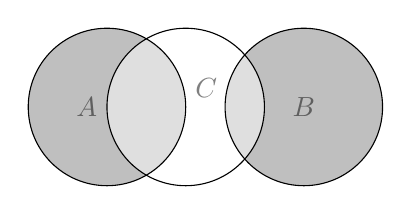
\begin{tikzpicture}
                \begin{scope}[shift={(3cm,-5cm)}, fill opacity=0.5]
                    \fill[gray] (0,0) circle (1);
                    \fill[gray] (2.5,0) circle (1);
                    \fill[white] (1,0) circle (1);
                    \draw (0,0) circle (1) node [left] {$A$};
                    \draw (2.5,0) circle (1) node {$B$};
                    \draw (1,0) circle (1) node [above right] {$C$};
                \end{scope}
            \end{tikzpicture}
    \end{enumerate}
    \textbf{2.10}
        \begin{enumerate}
            \item $S = \{NNN, NNF, NFN, NFF, FNN, FNF, FFN, FFF\}$
            \item $E = \{NFF, FNF, FFN, FFF\}$
            \item The second river is always safe to fish.
        \end{enumerate}
    \textbf{2.14}
        \begin{enumerate}
            \item $A\cup C = \{0, 2, 3, 4, 5, 6, 8\}$
            \item $A\cap B = \{\emptyset\}$
            \item $C' = \{0, 1, 6, 7, 8, 9\}$
            \item $(C'\cap D)\cup B = \{1, 3, 5, 6, 7, 9\}$
            \item $(S\cap C)' = \{0, 1, 6, 7, 8, 9\}$
            \item $A\cap C \cap D' = \{2, 4\}$
        \end{enumerate}
    \textbf{2.16}
        \begin{enumerate}
            \item $M\cup N = \{x \mid 0 < x < 9\}$
            \item $M\cap N = \{x \mid 1 < x < 5\}$
            \item $M'\cap N\ = \{x \mid 9 < x < 12\}$
        \end{enumerate}
    \textbf{2.22}\\
        $8 \cdot 3 = 24$ classifications\\\\
    \textbf{2.26}
        \begin{enumerate}
           \item $\binom{7}{5}$ = 21 ways
           \item $\binom{5}{3}$ = 10 ways
        \end{enumerate}
    \textbf{2.28}\\
        $5 \cdot 3 \cdot 2$ = 30 different ways\\\\
    \textbf{2.30}\\
        $9^2$ = 72 ways\\\\
    \textbf{2.34}
        \begin{enumerate}
            \item $7! = 5040$
            \item $6! = 720$
        \end{enumerate}
    \textbf{2.38}
        \begin{itemize}
            \item $8! = 40320$
            \item $4!\cdot 2^4 = 384$
            \item $4!\cdot 4! = 576$
        \end{itemize}
    \textbf{2.46}\\
        $\frac{9!}{3!4!2!} = 1260$\\\\
    \textbf{2.50}
        \begin{itemize}
            \item $P(A) = \frac{10}{36}$
            \item $P(C) = \frac{12}{36}$
            \item $P(A\cap C) = \frac{7}{36}$
        \end{itemize}
    \textbf{2.52}
        \begin{itemize}
            \item $210 - 122 = 88$\\
                $\frac{88}{500}$
            \item $83 - 52 = 31$\\
                $\frac{31}{500}$
            \item $500 - (210 + 216 - 97) = 171$\\
                $\frac{171}{500}$
        \end{itemize}
    \textbf{2.56}
        \begin{itemize}
            \item $0.25 + 0.17 - 0.15 = 0.27$
            \item $1 - (0.25 + 0.17 - 0.15) = 0.73$
        \end{itemize}
    \textbf{2.58}
        \begin{itemize}
            \item $\frac{5}{36}$
            \item $\frac{10}{36}$
        \end{itemize}
    \textbf{2.64}
        \begin{itemize}
            \item $1 - 0.42 = 0.58$
            \item $1 - 0.04 = 0.96$
        \end{itemize}
    \textbf{2.74}\\
    \textbf{2.80}\\
    \textbf{2.86}
    \begin{enumerate}
        \item fill
        \item fill
    \end{enumerate}
    \textbf{2.90}\\
    \textbf{2.92}\\
    \textbf{2.96}\\
    \textbf{2.98}\\
    \textbf{2.104}\\
    \textbf{2.118}\\
    \textbf{2.124}\\
    
\end{document}